\chapter{Discussion}
This chapter discusses the results of the project. If there were any specific problems or choices in implementation which was made, and why.

\section{Hardware}
There is very little, if any, official documentation available regarding the specifics of the hardware used in the Game Boy. While this complicates emulator development, there are members of the community who have dedicated a lot of resources into providing accurate documentation on the hardware. Among these are two of the co-authors of PanDocs \cite{pandocs}, Gekkio \cite{Gekkio.fi} and Antonio Niño Díaz \cite{AntonioND}. Both of which are also authors of their own very detailed documentations of the Game Boy, the ``Game Boy: Complete Technical Reference'' \cite{CompleteTechnicalReference} and ``The Cycle-Accurate Game Boy Docs'' \cite{TCAGBD} respectively. These two documents are based on tests written and ran on multiple units of the real hardware to ensure that they are testing correct behaviour, and thereby providing a way to reverse engineer the hardware. These sources, or sources similar to these, have therefore been central in the development of this emulator.

\subsection{The Central Processing Unit}
\label{sec:CPUDiscussion}
While implementing the CPU, a problem regarding the number of machine cycles an operation required was encountered. The problem was that the source used for the operation codes \cite{OpCodes}, which displays flags affected, number of bytes used and number of machine cycles, was not the same as used in Blargg's test ROMs \cite{Blargg}. As the test ROMs have been run on the real hardware and passed the tests, the team considered the test ROMs to be using the correct amount of cycles \cite{TestROMsResult}. A process similar to what Gekkio and Díaz applies in their testing.
\\\\
Looking at Blargg's test suite regarding the CPU tests, one might note that the emulator does in fact not pass all tests. Among the tests which it does not pass are the \texttt{interrupt\_time}, \texttt{mem\_timing} and \texttt{mem\_timing-2} \cite{Blargg}. As mentioned in section \ref{sec:resultsarchitecture}, the different units need to be synchronised and act in accordance with each other. There are indications that the reason for the tests failing is that it is possible for the CPU to execute too many machine cycles before allowing the other units to catch up or interrupts to intercept. Meaning that the current implementation of the CPU does not allow for timer updates mid-instruction. In hindsight, it is possible that the problems encountered as a result of this choice could have been avoided. One possible solution could be to allow the other units to catch up to the CPU mid-instruction every time it reads from or writes to memory.
\\

\begin{comment}


\begin{lstlisting}[language=C++,
caption = {Code displaying how the CPU executes an instruction and returns the number of machine cycles, whereafter the other units catch up by executing the same number of cycles.},
label = {step}]


void GameBoy::step(IVolumeController *vc){
    ...
    int cycles = this->cpu->update();
    ppu->update(cycles);
    apu->update(cycles, vc);
    timer->update(cycles);
    cartridge->update(cycles);
    ....
    }
\end{lstlisting}
\end{comment}

\subsection{The Memory Management Unit}
Early in the development all memory and registers were located directly in the MMU class. 
When first implementing the PPU it always needed to ``fetch'' the registers it needed from the MMU to continue to do its job.
This made it clear that it would be better to make the different device classes keep their own registers.
With this change it was necessary but also natural to make use of individual read and write functions for each device, which in turn would be called from the main read/write function located in the MMU class.
\\\\
In the memory map, seen in figure \ref{fig:memory-map}, there are some areas which are empty.
Although Nintendo says use of these areas are prohibited they still have a specific behaviour confirmed on all official hardware \cite{pandocsechoram}.
The seemingly empty range \texttt{0xE000}-\texttt{0xFDFF} is by the community called ``Echo RAM'' and is on the original hardware mapped to the actual RAM addresses.
For example, writing a value to address \texttt{0xE001} would have the same effect as writing to the address \texttt{0xA001}. Same goes with reading values.
We have chosen to not implement this behaviour mainly because it is prohibited by Nintendo and is expected to be unused in licensed games. 
Additionally, this behaviour does not add any functionality that cannot be achieved by other means.
Furthermore, if it is used in unlicensed games it is easily implemented down the line.  
\\\\
The choice to only implement two different MBCs was made because the most popular games make use of these MBCs. 
Implementing more MBCs would yield less return for the time spent and time was therefore put into other areas that felt more important. Also, as previously mentioned, a modular approach was taken when implementing MBCs, making it easy to implement in the future if wanted.
\\\\
Limiting access to different memory areas under certain circumstances has not been implemented, as this is expected to be respected by game developers. For example, during a DMA-transfer the CPU, on the original hardware, is limited to only access HRAM during that period.

\subsection{The Pixel Processing Unit}
As mentioned both in sections \ref{sec:CPUDiscussion} and \ref{sec:PPU}, the different units are synchronised with the CPU by supplying the other units with the number of cycles the CPU has consumed after having completed each instruction. This made simulating the PPU accurately impossible and the approach of drawing one scanline at a time was instead chosen. The biggest limitation resulting from this choice is that the emulator does not support writing to PPU hardware registers mid-scanline. This results in graphical glitches in a few games, but is not a problem for a vast majority of games. However, the emulator supports writing to hardware registers between scanlines, enabling visual effects such as the one shown in figure \ref{fig:flappyboy}:


\begin{figure}[H]
\centering
\begin{subfigure}{.5\textwidth}
  \centering
  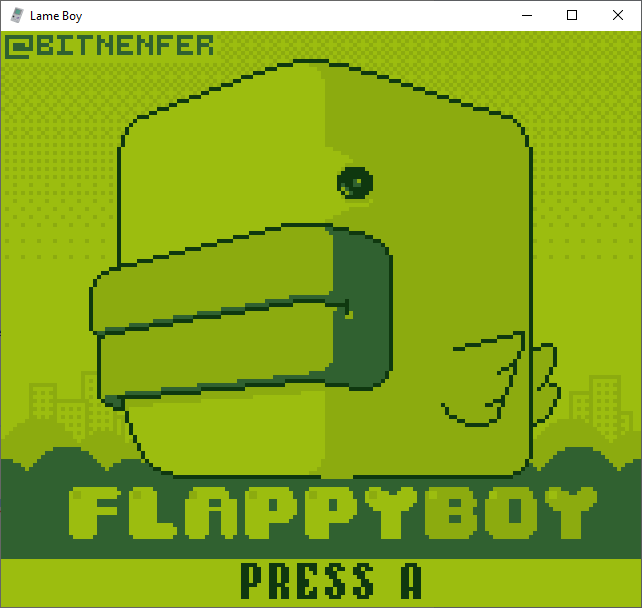
\includegraphics[width=0.9\linewidth]{figures/PPU/Flappyboy_normal.PNG}
  %\caption{Figure displaying the emulator passing Blargg's test checking the correctness of the CPU instructions.}
  %\label{fig:cpu_instrs}
\end{subfigure}%
\begin{subfigure}{.5\textwidth}
  \centering
  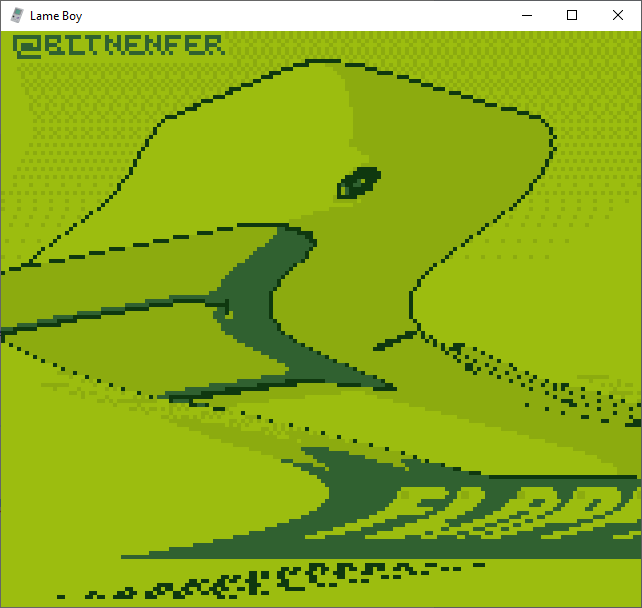
\includegraphics[width=0.9\linewidth]{figures/PPU/Flappyboy_distorted.PNG}
 % \caption{Figure displaying the emulator passing Blargg's test checking the correctness of the CPU timing.}
  %\label{fig:instr_timing}
\end{subfigure}
\caption{The starting screen of the game Flappyboy. From left to right, its original form and its distorted form achieved by writing to the SCX and SCY registers between scanlines. From \cite{FlappyBoy}. Screenshot by authors, used with permission.}
\label{fig:flappyboy}
\end{figure}   

The decision to render the image scanline by scanline was made as it supported the aforementioned wobble effect and other visual effects, while still being achievable within the given time frame. To support writing to hardware registers mid-scanline would require a much more accurate simulation of the original PPU and was not feasible in the allotted time.\\
\\
Another difference between the emulator and the original PPU is that the emulator does not limit the CPU's access to VRAM and OAM. This could lead to bugs in games where the developers have not ensured that the CPU has access to VRAM or OAM before reading or writing to these memory areas.\\
\\
All in all, graphical glitches are few and far in between and the PPU must therefore be considered correctly implemented within the scope of the project.

\subsection{The Audio Processing Unit}
Implementing sound was initially considered out of scope, as it was deemed too complex and would take too much time to implement. Therefore any progress made in this regard is seen as exceeding the initial expectations. As the development of the other parts progressed faster than expected, there was time to spare which allowed for the implementation of the APU.
\\\\
%Creating a small separate project, only for checking out the the OpenAL library what helpful since it allowed us to only keep the code we wanted. It also allowed us to check that the library worked for all group members which used different platforms.
Only implementing one channel at a time was a good strategy as once the first channel had been implemented, it was easy to implement more. The biggest difference between  the sound channels was how the audio was generated. Thankfully they could be implemented similarly without changing much but the audio data provided to the OpenAL API.
\\\\
However, the devil is in the details, and for the APU there are a lot of them. There have been several issues where sound continues to play when it should have been muted, sound beginning to play from nowhere when it is not suppose to etc. Most of these issues have been resolved, but there are still existing issues with some games where the audio does not play at all.
\\\\
The room for improvement is also apparent in the results of running Blargg's \texttt{dmg\_sound} \cite{Blargg} test ROM which, as seen in figure \ref{fig:blargg_dmg_sound}. Almost all tests fail due to these small details not being implemented. On the other hand, having sound implemented in any form and in some ways working as expected, is exceeding the initial expectations.

\section{Accuracy}
One thing to always consider when discussing the development of emulators is the accuracy of the emulation, and specifically how accurate the emulator aims to be. Some developers choose to try to emulate the exact behaviour of the hardware, including what today could be considered bugs, flaws, or mistakes. Others seize the opportunity and correct some behaviour of the emulator which they deem incorrect or faulty.

\subsection{Compromises}

Given the scope and the time spent on this project, this emulator had to be made with some compromises between accuracy and progress. Assuming the aim would have been to be as accurate as possible, a lot more research would have had to been done, and implementation could and would have had to be planned more carefully. On the other hand, many of the systems are implemented with the intention of making the emulator extensible and easy to further develop.
\\\\
One of the compromises made was considering the choice of further developing the CPU, making it more accurate and passing more test ROMs, like Blargg's interrupt timing test \cite{Blargg}, or attempting to implement sound. Adding sound to the emulator would increase the overall impression and feeling of the emulator, while there is no guarantee that making the CPU more accurate would increase the user experience in any way. One might even argue that implementing additional features such as saves, a functional GUI and other quality of life features yields a better overall impression than improving the accuracy of the emulation. Therefore the choice fell on trying to implement sound and other, smaller, features.

\subsection{Vital and auxiliary components}

Some components of the Game Boy are more important than others, which means these have to be more accurately emulated than auxiliary components. The most vital component to be emulated accurately is the CPU since it is the central component of both the Game Boy and the emulator. Any bugs caused by the CPU may result in obscure behaviours which can be close to impossible to debug. Getting Blargg's \texttt{cpu\_instrs} and \texttt{instr\_timing} \cite{Blargg} test ROMs working was therefore highly prioritised in order to validate the accuracy of the CPU and avoid any of these potential bugs.
\\\\
The APU, which on the other hand could be considered an auxiliary component, was not given the same attention in regards to accuracy as the consequences of having a defective APU is not as severe. The worst thing that could happen with the APU is the absence, or constant presence, of sound, but all other parts of the emulator would still work as intended. This is because, in contrast to the CPU, no other component strictly relies on the APU to perform its function accurately. The results of this approach to accuracy is visible in figure \ref{fig:blargg_dmg_sound} which shows only test \texttt{06} passing when running Blargg's \texttt{dmg\_sound} \cite{Blargg} APU test ROM.


\section{Ethics}
As mentioned in section \ref{sec:introEthics}, the emulation of a proprietary product comes with both ethical and legal complications, some of which are discussed in this section.
\label{sec:Ethics}
\subsection{Legality of emulators vs. ROMs}
Most digital copyrighted material have some sort of controversy around them. Gaming consoles and their respective emulators are no different. Like with most subjects touching on potential piracy and copyright infringement, there is a huge grey zone whether or not something is legal or illegal, and subsequently if something is right or wrong. 

\subsection{The emulator}
The creation of an emulator is generally not illegal as long as no proprietary code is used \cite{emulatorLegal}. This is mainly because the emulator itself does not necessarily have to contain any proprietary code to replicate the original console. Some consoles do have proprietary code in their BIOS, however this can usually be avoided either by flashing a BIOS legally, or creating a custom BIOS. 

\subsection{The Boot ROM}
As previously mentioned, the boot ROM initialises the Game Boy while scrolling down the Nintendo logotype, something which might seem like a banality at first. However, this means that the official boot ROM cannot be used in emulators as it uses both copyrighted code, and displays a copyrighted logo. Additionally, on the original hardware the Game Boy enforces that any game run on the Game Boy has to contain the Nintendo logotype \cite{GBTROM}. This is done by comparing the logotype data stored on the boot ROM with data stored on the inserted game. If this data does not match, the Game Boy locks itself up. This allows Nintendo to control what is released to the platform, as any game released for the Game Boy has to contain copyrighted material to run on the official hardware, and therefore needs the approval of Nintendo \cite{GBTROM}.

\subsection{The ROMs}
Copyright laws differ from country to country, which complicates the matter further. In the United States (US), there are multiple cases in court regarding the creation of emulators and distribution of ROMs \cite{euRomLegal}. In the European Union (EU), however, it is more difficult to find actual court cases around emulation, which creates confusion for people without a legal education. The European Parliamentary Research Service has documentation which describes the copyright laws in the EU \cite{euCopyright}. This documentation is on the other hand not as easily interpreted as pre-existing cases, of which there seem to be very few using EU law.
\\\\
Due to the difficulty of interpreting the EU law as a layperson when discussing the legality of ROMs, the US law is usually referred to. Furthermore, according to US law the ROMs themselves are in a bit of a grey zone \cite{romLegal}. Making back ups of game cartridges one already owns is completely legal under the right circumstances and for the right purposes according to US copyright laws \cite{section117}. Selling or distributing said copies is illegal and counts as copyright infringement, and so does downloading other people's copies. The main legal way to get a playable version of an existing game's ROM seems to be through making your own copy of that specific game, which you must already own. Piracy and copyright laws do vary from country to country, and there is continuous debate online whether or not these laws are for the greater good or not \cite{emulatorPodcast}. Furthermore, it is not always clear which country's laws are to be followed, since the company who owns the copyright might not be based in the same country as the person using their content.

%Copyright laws differ from country to country, which complicates the matter further. In the United States (US), there are multiple cases in court regarding the creation of emulators and distribution of ROMs \cite{euRomLegal}. In the European Union (EU), however, it is more difficult to find actual court cases around emulation, which creates confusion for people without a legal education. The European Parliamentary Research Service has documentation which describes the copyright laws in the EU \cite{euCopyright}. Although this documentation is not as easily interpreted as preexisting cases, of which there seem to be very few. The ROMs themselves are in a bit of a grey zone \cite{romLegal}. Making back ups of game cartridges one already owns is completely legal under the right circumstances and for the right purposes according to US copyright laws \cite{section117}. Selling or distributing said copies is illegal and counts as copyright infringement, and so does downloading other people's copies. The main legal way to get a playable version of an existing game's ROM seems to be through making your own copy of that specific game, which you must already own. Piracy and copyright laws do vary from country to country, and there is continuous debate online whether or not these laws are for the greater good or not \cite{emulatorPodcast}. Furthermore, it is not always clear which country's laws are to be followed, since the company who owns the copyright might not be in the same country as the person using their content.

\subsection{Test-ROMs}
%On the topic of of developing an emulator which has the ability to emulate copyright-infringing ROMs the question regarding the acquisition of legal game ROMs which are usable for testing.

If game ROMs are not acquirable for some reason, there are a multitude of test-ROMs online that are available to make sure the emulator and its parts work as intended \cite{testROMs}. These are free to use and has benefited the troubleshooting of this project immensely without any risk for potential copyright infringement. There are also games developed by the community, i.e. non-proprietary ROMs, specifically for emulators which have been used for testing.


\subsection{Sharing knowledge}
By creating an emulator for an old console one gets to thoroughly understand how the very basic components of a gaming system work together to create a complete console. By making the emulator's source code available publicly, it might help increase the knowledge of these types of systems among students, enthusiasts and developers alike. As long as no proprietary code is shared, there is no obvious way this could harm anyone. If the Game Boy was not discontinued one could argue that an emulator would deter people from buying an expensive console. However, since the Game Boy is no longer being sold, that risk is effectively eliminated. On the contrary, finding an emulator might even contribute to further interest in Nintendo products which would most likely benefit them.


\subsection{Gaming history preservation}
One of the main pro-emulation arguments is that of historic preservation. The Game Boy was made with hardware that degrades over time, which limits each units lifetime. Ever since the product was discontinued in 2003 \cite{gameBoyDisc} people have been urging to save what many believes to be one of the greatest gaming products ever released. Much like museums would save objects from historical events, Game Boy emulators and ROM archiving could be seen as a kind of digital museum where the soon to be lost hardware is forever stored. Several games for the Game Boy are no longer being sold, and acquiring a used copy becomes increasingly more difficult with time. This makes retro game emulation for historic preservation quite an attractive option for a lot of people. However the legal situation around emulators is very much a grey zone, which makes justifying an emulator for this purpose much more difficult. Creating an emulator would definitely contribute to increased historic preservation, however through incorrect use it could also be a tool for playing illegal copies of games.

\subsection{Console Classix}
An example of a company which has tried to make old ROMs playable to the public is Console Classix \cite{romLegal}. The idea is to rent their games through a client-server solution to make the games playable on a home PC. Although they have received a letter from Nintendo regarding their business \cite{letterFromNintendo}, no legal action has been taken since. Console Classix's defence is that they, unlike illegal ROM sharing websites, do not publish the ROMs publicly but rather provide limited access to them with a subscription method. By sending the ROM images directly from the server to the client's RAM, the game effectively disappears from the client when they stop playing, which would prevent any permanent distributing from happening. Additionally, they do not rent more copies out than they own, therefore it is difficult to build a case around copyright infringement as well. This is a great example of using an emulator seemingly legally to still fill the purpose of historic preservation, while simultaneously providing a way to play retro games for those subscribed to their service.
%\section{Evaluating KPIs?}


\section{Future Work}
Going forward, there are numerous ways to improve the emulator. Initially, one could work on improving its accuracy, ensuring that more games are playable without any unintended behaviour, for example by continuing to work towards passing more test ROMs. Furthermore, there are many additional features regarding quality of life which could be implemented, such as quick saves, shortcuts for commands etc. One could even develop a debugger/disassembler for the emulator or modularise the code further in an effort to emulate multiple systems within one emulator.% Most of these things have already been done, for example by BGB \cite{BGB}.
\\\\
Furthermore most emulators are created for one of three purposes: they either aim to provide ways to play old games, a historical documentation of a product which is at risk to be lost to time or as a form of learning experience. Most of which results in a code base which is more or less cluttered, either due to inexperience in the field, that the code bases are very big, or due to the fact that they aim to reproduce exact behaviour of hardware. Additionally, due to the fact that there is no official documentation from Nintendo regarding the Game Boy, most emulators will be dependent on people such as Gekkio \cite{Gekkio.fi} or Díaz \cite{TCAGBD} as most people do not have the technical competence or resources available to reverse engineer the hardware. This results in the available emulators being quite homogeneous, where most emulators are built using the same source material. Most will probably even use the same tests to check the emulator's accuracy compared to the real hardware. As a developer of an emulator it is therefore highly unlikely that you bring something new to the table.
\\\\
One might therefore ask oneself if there is any academic interest in such a product. One could then consider the fact that video games are extremely popular among the general population. This is something which could be leveraged into piquing an interest for low-level programming and hardware through the use of emulator development. This could, for instance, be done by providing an emulator which has a clear structure, is effectively modularised and commented. The purpose would not be to make the most accurate or the fastest emulator, but rather to provide a clear point of reference for the interaction between hardware and software. This emulator could then work as an inspiration for other potential developers, creating a base for further learning. 